\documentclass[12pt]{ltjsarticle}
\usepackage{amsmath,ascmac,amssymb,mathtools,siunitx,diffcoeff,inputenc}
\usepackage{mygraphics}
\graphicspath{{./images/}}
\usepackage[oldfont,exchangeupit]{unicommand}
\usepackage{subfiles}

%% options %%
\renewcommand{\headfont}{\bfseries}
% \numberwithin{equation}{section}
% \renewcommand*\abstractname{}
% \setlength{\parindent}{0pt}

\begin{document}
\title{ダイマー模型による2次元Ising模型の厳密解}
\author{政岡凜太郎}
\date{最終更新: 2024年12月10日}
\maketitle

2次元Ising模型の厳密解についてはOnsagerによる解の他にMajoranaフェルミオンを用いる方法やダイマー模型を用いる方法が知られている。
このノートではダイマー模型による解法について解説する。

\subsection*{
    問題設定
}
IsingモデルのHamiltonianは
\begin{align}
    H{σ} = -J∑_{⟨i,j⟩}σ_iσ_j
\end{align}
と書かれる。
$σ_i$は2次元正方格子の頂点上で定義されるスピン変数であり、
$±1$の値を取る。
$⟨i,j⟩$は最近接格子点を表す。
また分配関数は、
\begin{align}
    Z = ∑_{\{σ\}}∏_{⟨i,j⟩}ℯ^{βJσ_iσ_j}
\end{align}
2次元正方格子の頂点の総数を$L²$とおく。
このとき辺の総数は$2L²$となる。
サイトあたりの自由エネルギー$f$は
\begin{align}
    -βf = \lim_{L → ∞}÷1{L²}\ln Z
\end{align}
によって計算される。
$L → ∞$の極限をとるため、
格子の境界条件についてはあまり気にしないことにする。

以下では2次元Isingモデルの厳密解として、
Isingモデルを対応するダイマーモデルに変換して、
その数え上げをPfaffianによって計算するという方法を紹介する。

% \subsection*{
%     高温展開
% }
% まず、2次元Isingモデルに対する高温展開を導入する。
% $K ≔ βJ$とおく。
% $σ_i = ±1$から、
% \begin{align}
%     ℯ^{Kσ_iσ_j}
%     = \cosh(Kσ_iσ_j) +\sinh(Kσ_iσ_j)
%     = \cosh K + σ_iσ_j\sinh K
% \end{align}
% と変形することができる。これを$\cosh K$で割って、
% \begin{align}
%     ÷{ℯ^{Kσ_iσ_j}}{\cosh K}
%     = 1 + σ_iσ_j\tanh K
%     = ∑_{λ_{⟨i,j⟩} = 0,1}(σ_iσ_j\tanh K)^{λ_{⟨i,j⟩}}
%     \label{local weight}
% \end{align}
% と書く。
% ここで、分配関数を$(\cosh K)^{2L²}$で割ったものを考えよう。
% これは(\ref{local weight})を掛け合わせて、
% あらゆるスピンの配位について和をとったものである。
% \begin{align}
%     ÷Z{(\cosh K)^{2L²}}
%     = ∑_{\{σ\}}∑_{\{λ\}}
%         ∏_{⟨i,j⟩}(σ_iσ_jq)^{λ_{⟨i,j⟩}}
% \end{align}
% ただし、$q = \tanh K$とおいた。
% $σ_i$についての和を先に取ると、
% \begin{align}
%     ∑_{σ_i = ±1}σ_i^n = \begin{cases}
%         2 & (n =\𝚞{even})\\
%         0 & (n =\𝚞{odd})
%     \end{cases}
% \end{align}
% より、任意の頂点に対して偶数個の$σ_i$があるような項以外は全て消える。
% つまり、任意の頂点$i$に対して接する$λ_{⟨i,j⟩}$の合計は必ず偶数になる。
% これは$λ_{⟨i,j⟩}=1$となる辺がサイクルを作ることを意味する。
% したがって、
% \begin{align}
%     ÷Z{(\cosh K)^{2L²}}
%     = 2^{L²} ∑_{\𝚝{closed curve}} q^{(\𝚝{length})}
% \end{align}
% と書ける。
% ただし、和は格子上の任意のサイクルについての和であり、
% $(\𝚝{length})$は$λ_{⟨i,j⟩} = 1$となる辺の総数を表す。
% サイクルという言葉は任意の頂点に対して偶数本の辺が接するグラフというのを短く言い換えただけに過ぎない。
% サイトあたりの自由エネルギーは
% \begin{align}
%     -βf = ÷1{L²}\ln Z
%     = \ln(2\cosh²K)
%     +÷1{L²}\ln(∑_{\𝚝{closed curve}} q^{(\𝚝{length})})
%     \label{free energy with loop}
% \end{align}
% により与えられる。

\subsection*{
    双対格子における分配関数
}
Isingモデルを双対格子で考えてみよう。
すなわち、正方格子の各面にスピン変数$σ = ±1$を割り当てる。
スピンが揃った強磁性状態のエネルギー$E = -2JL²$を基準に取ると、
スピンが揃った領域の中ではエネルギーは$0$で、
領域の境界に$2J×\𝚝{(境界の長さ)}$だけエネルギーが発生する。

閉曲線を与えると、それを境界にもつスピン配位が存在する。
ただし、スピンを全て反転しても同じ境界が得られるから、
境界から2通りのスピン配位が得られる。
ここから、分配関数を正方格子上の閉曲線についての和として表すことができる。
\footnote{
    周期境界条件を課す場合にドメインウォールとしては得られない閉曲線があり得るが、
    そのような場合の寄与は熱力学極限では無視できる。
}
$q ≔ ℯ^{-2βJ}$とおくと、
\begin{align}
    Z = 2q^{-2L²}∑_\𝚝{closed curve}q^{(\𝚝{length})}
\end{align}
と書ける。
ただし、$(\𝚝{length})$は閉曲線の長さを表す。
サイトあたりの自由エネルギーは
\begin{align}
    -βf = -2\ln q + ÷1{L²}\ln(∑_\𝚝{closed curve}q^{(\𝚝{length})})
    \label{free energy with loop}
\end{align}
となる。ここで$\ln 2/L²$は熱力学極限で無視できるので省いた。

\subsection*{
    ダイマーモデルへの変換
}
ダイマー(二量体)とは、2つの頂点の組のことである。
グラフ理論の文脈でマッチングと呼ばれることも多い。
ダイマーモデルの分配関数は、
グラフの頂点を2つずつに分けるような方法について、
重み付きで足し上げることで得られる。

Isingモデルは以下のようにダイマーモデルに変換できる。
まず、正方格子の全ての頂点を、4点からなる完全グラフ$K₄$に置き換える。
元の正方格子に含まれる辺はexternalな辺と呼び、
完全グラフに含まれる辺をinternalな辺と呼ぶことにする。
\begin{figure}[H]
    \centering
    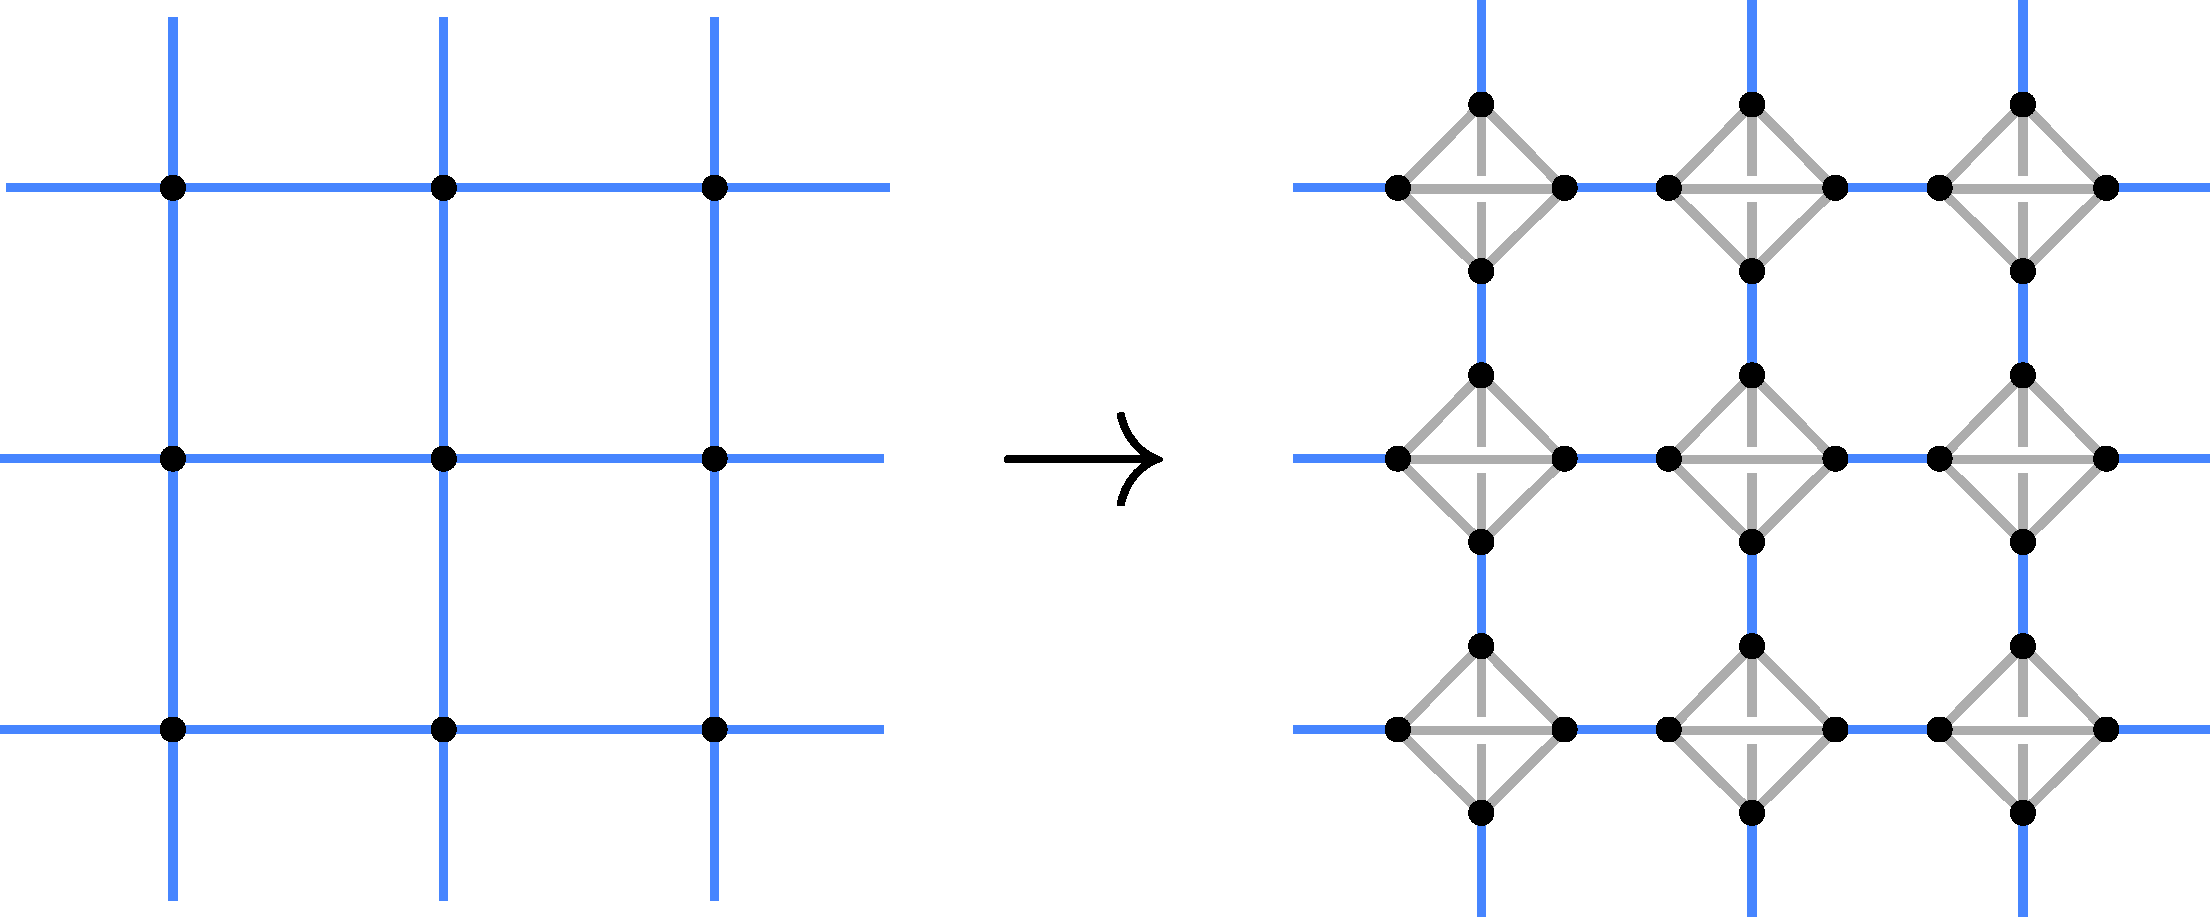
\includegraphics[width=0.7\hsize]{../images/lattice_modification.pdf}
\end{figure}
この格子の辺に標準となる向きをつけ、以下のような重みを設定する。
\begin{figure}[H]
    \centering
    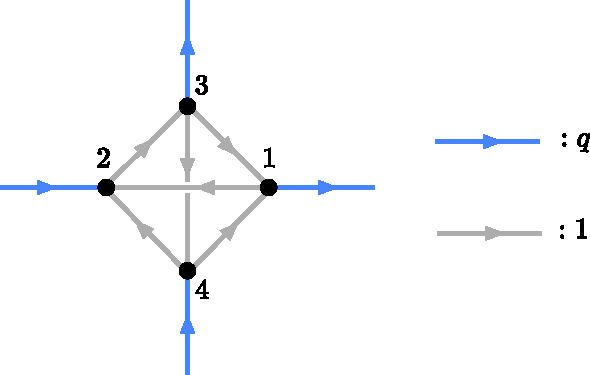
\includegraphics[width=0.4\hsize]{../images/vertex.pdf}
\end{figure}
頂点$i$から頂点$j$への矢印が重み$w_{ij}$を表すとする。
また$w_{ji} = -w_{ij}$とする。
externalな矢印の重みは$q$とし、internalな矢印の重みは$1$とする。

頂点の置換$σ ∈ S_{4N}$を与えると、
ダイマーへの分割は
\begin{align}
    {\{σ(1),σ(2)\},…,\{σ(4N-1),σ(4N)\}}
\end{align}
と表される。
ただし$\{⋯\}$は集合を表す括弧であり、要素の順序は問わない。
したがって$S_{4N}$の元がそれぞれ異なるダイマーを与えるわけではない。
このダイマー配位に対する重みは
\begin{align}
    \sign(σ)w_{σ(1)σ(2)}⋯w_{σ(4N-1)σ(4N)}
\end{align}
とする。
ここで、$\sign(σ)$はダイマーを不変に保つ置換に対して重みが不変になるように導入した符号因子である。
( $\sign(σ)$は$w_{ij}↔w_{ji}$に対して符号を変え、
$w_{ij}w_{kl}↔w_{kl}w_{ij}$に対して符号を保つ。)
ダイマーモデルの分配関数は
\begin{align}
    Z_{\𝚞{Dimer}}
    &
    = ∑_{\𝚝{dimer covering}}    \sign(σ)w_{σ(1)σ(2)}⋯w_{σ(4N-1)σ(4N)}
    \∅ & 
    ≕ \Pf 𝒲
    = √{\det 𝒲}
\end{align}
で与えられる。ここで$𝒲$は$w_{ij}$を成分とする行列である。
また$(\Pf 𝒲)² = \det 𝒲$の証明については省略する。

修正された格子上でのダイマーが与えられると、
externalな辺のみを取り出すことで正方格子上の閉曲線が得られる。
逆に正方格子上の閉曲線をexternalな矢印に移し、
ペアのいない余っている頂点をinternalな矢印で結ぶことで、
修正された格子上でのダイマーが得られる。
ただし矢印は全て標準の向きを向いているとする。
頂点にexternalな辺が4つ接するとき、または2つ接するとき、
internalな辺の足し方は一意に定まる。
しかし、頂点にexternalな辺が接しない場合、
internalな辺の足し方が以下の3通り存在することが問題になる。
\begin{figure}[H]
    \centering
    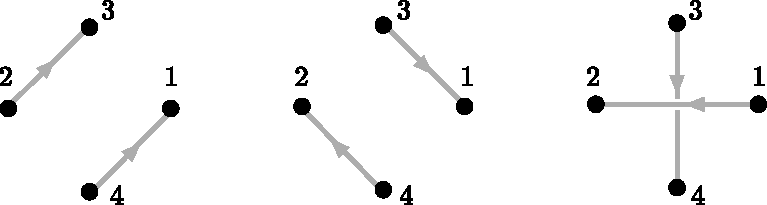
\includegraphics[width=0.5\hsize]{../images/3vertices.pdf}
\end{figure}
実は、この点については気にする必要がない。
なぜならば、2個目と3個目は符号が反対のため常に相殺するからである。
実際、2個目と3個目の重みの比をとると、
\begin{align}
    ÷{\sign(4231)⋅1⋅1}{\sign(1234)⋅1⋅1} = -1
\end{align}
となる。
\subsection*{
    符号の追跡
}
前節では閉曲線とダイマーの対応関係を導入した。
ダイマーモデルにおける重みの絶対値は、
externalな辺の数$=(\𝚝{length})$によって、$q^{(\𝚝{length})}$と書けるので、
この関係は分配関数のレベルで成り立つように思える。
しかし、完全な対応関係を示すためには異なるダイマーに対して置換の符号が整合するかを確認する必要がある。
基本となるのは、以下のようなダイマーの変形である。
% \begin{figure}[H]
%     \centering
%     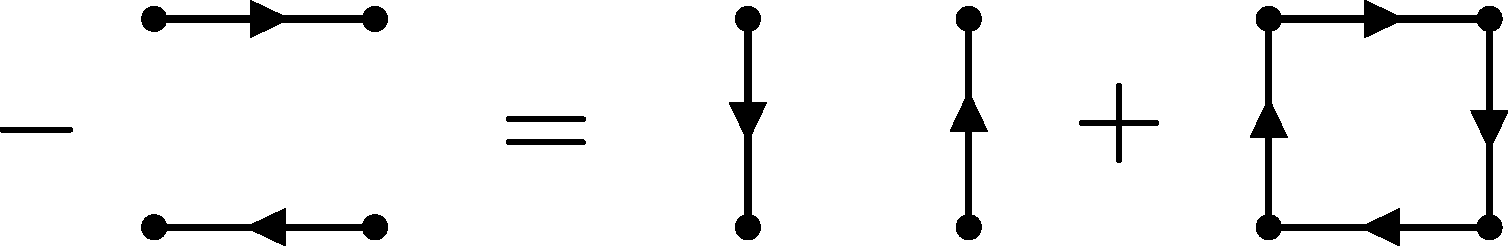
\includegraphics[width=0.4\hsize]{../images/normal_transformation.pdf}
% \end{figure}
\begin{align}&
    {(i₁,i₂),(i₃,i₄),…,(i_{2l-1},i_{2l})} \∅
    &
    ↦ {(i_{2l},i₁),(i₂,i₃),…,(i_{2l-2},i_{2l-1})}
\end{align}
ただし、符号を考えたいので向きも含めて考えている。
これはダイマーを指定する置換$σ$に対して巡回置換
\begin{align}
    \(
        i₁&i₂&i₃&⋯&i_{2l} \\
        i_{2l}&i₁&j₂&⋯&i_{2l-1}
    \)
\end{align}
を作用させることに等しい。
これは奇置換だから、$\sign(σ)$は$-1$倍される。
1つのダイマーから出発して、巡回置換の導入と矢印の反転によって任意のダイマーを得ることができる。
そこで、以下のダイマーを基準に取ることにしよう。
\begin{figure}[H]
    \centering
    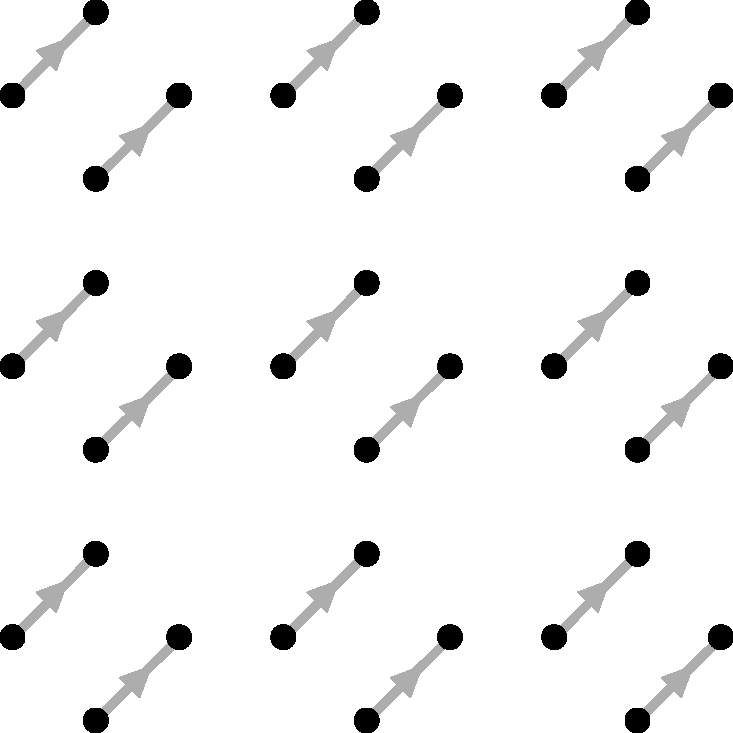
\includegraphics[width=0.25\hsize]{../images/standard_covering.pdf}
\end{figure}
ここから出発して任意のダイマーへ変形しようとするとき、
それらの差分
\footnote{
    ダイマーを$ℤ₂$係数ベクトルとみなして差をとる。
}
は偶数本の辺からなるいくつかのサイクルになる。
例えば以下のようなものである。
\begin{figure}[H]
    \centering
    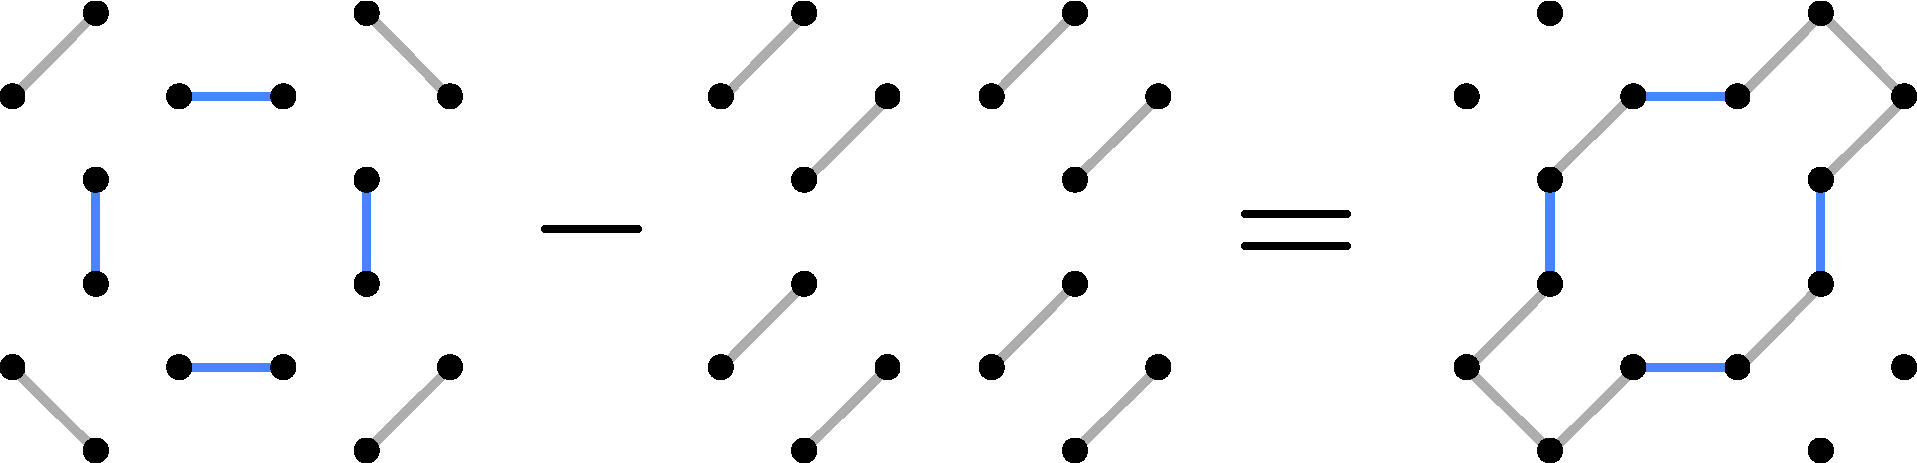
\includegraphics[width=0.5\hsize]{../images/loop.pdf}
\end{figure}
サイクルができることは、
ダイマーを2つ重ねると必ずある頂点が2つの頂点につながることから分かる。
また2つのダイマーからの辺が交互につながるので、サイクルは偶数本の辺を含む。
したがって、任意のダイマーは以下のように構成される。
\begin{itemize}
    \item 基準となるダイマーから出発する。
    \item 目的とするダイマーと基準となるダイマーとの差をとってサイクルを得る。
    \item このサイクルに沿って時計回りになるように、辺の向きを取り直す。
    \item サイクルに沿った巡回置換を使って、目的とするダイマーを構成する。
    \item 向きを標準の向きに直す。
\end{itemize}
これらのステップを通じた置換の符号が$+1$であれば良い。
巡回置換は必ず偶数のサイクルに対して行われるので、
符号は$-1$である。
したがって、
標準の向きからサイクルに沿う向きに矢印を反転したときの符号が$-1$であれば良い。
ここでサイクルの構成要素を列挙して矢印を反転する際の符号を調べると、
以下のようになる。
\begin{figure}[H]
    \centering
    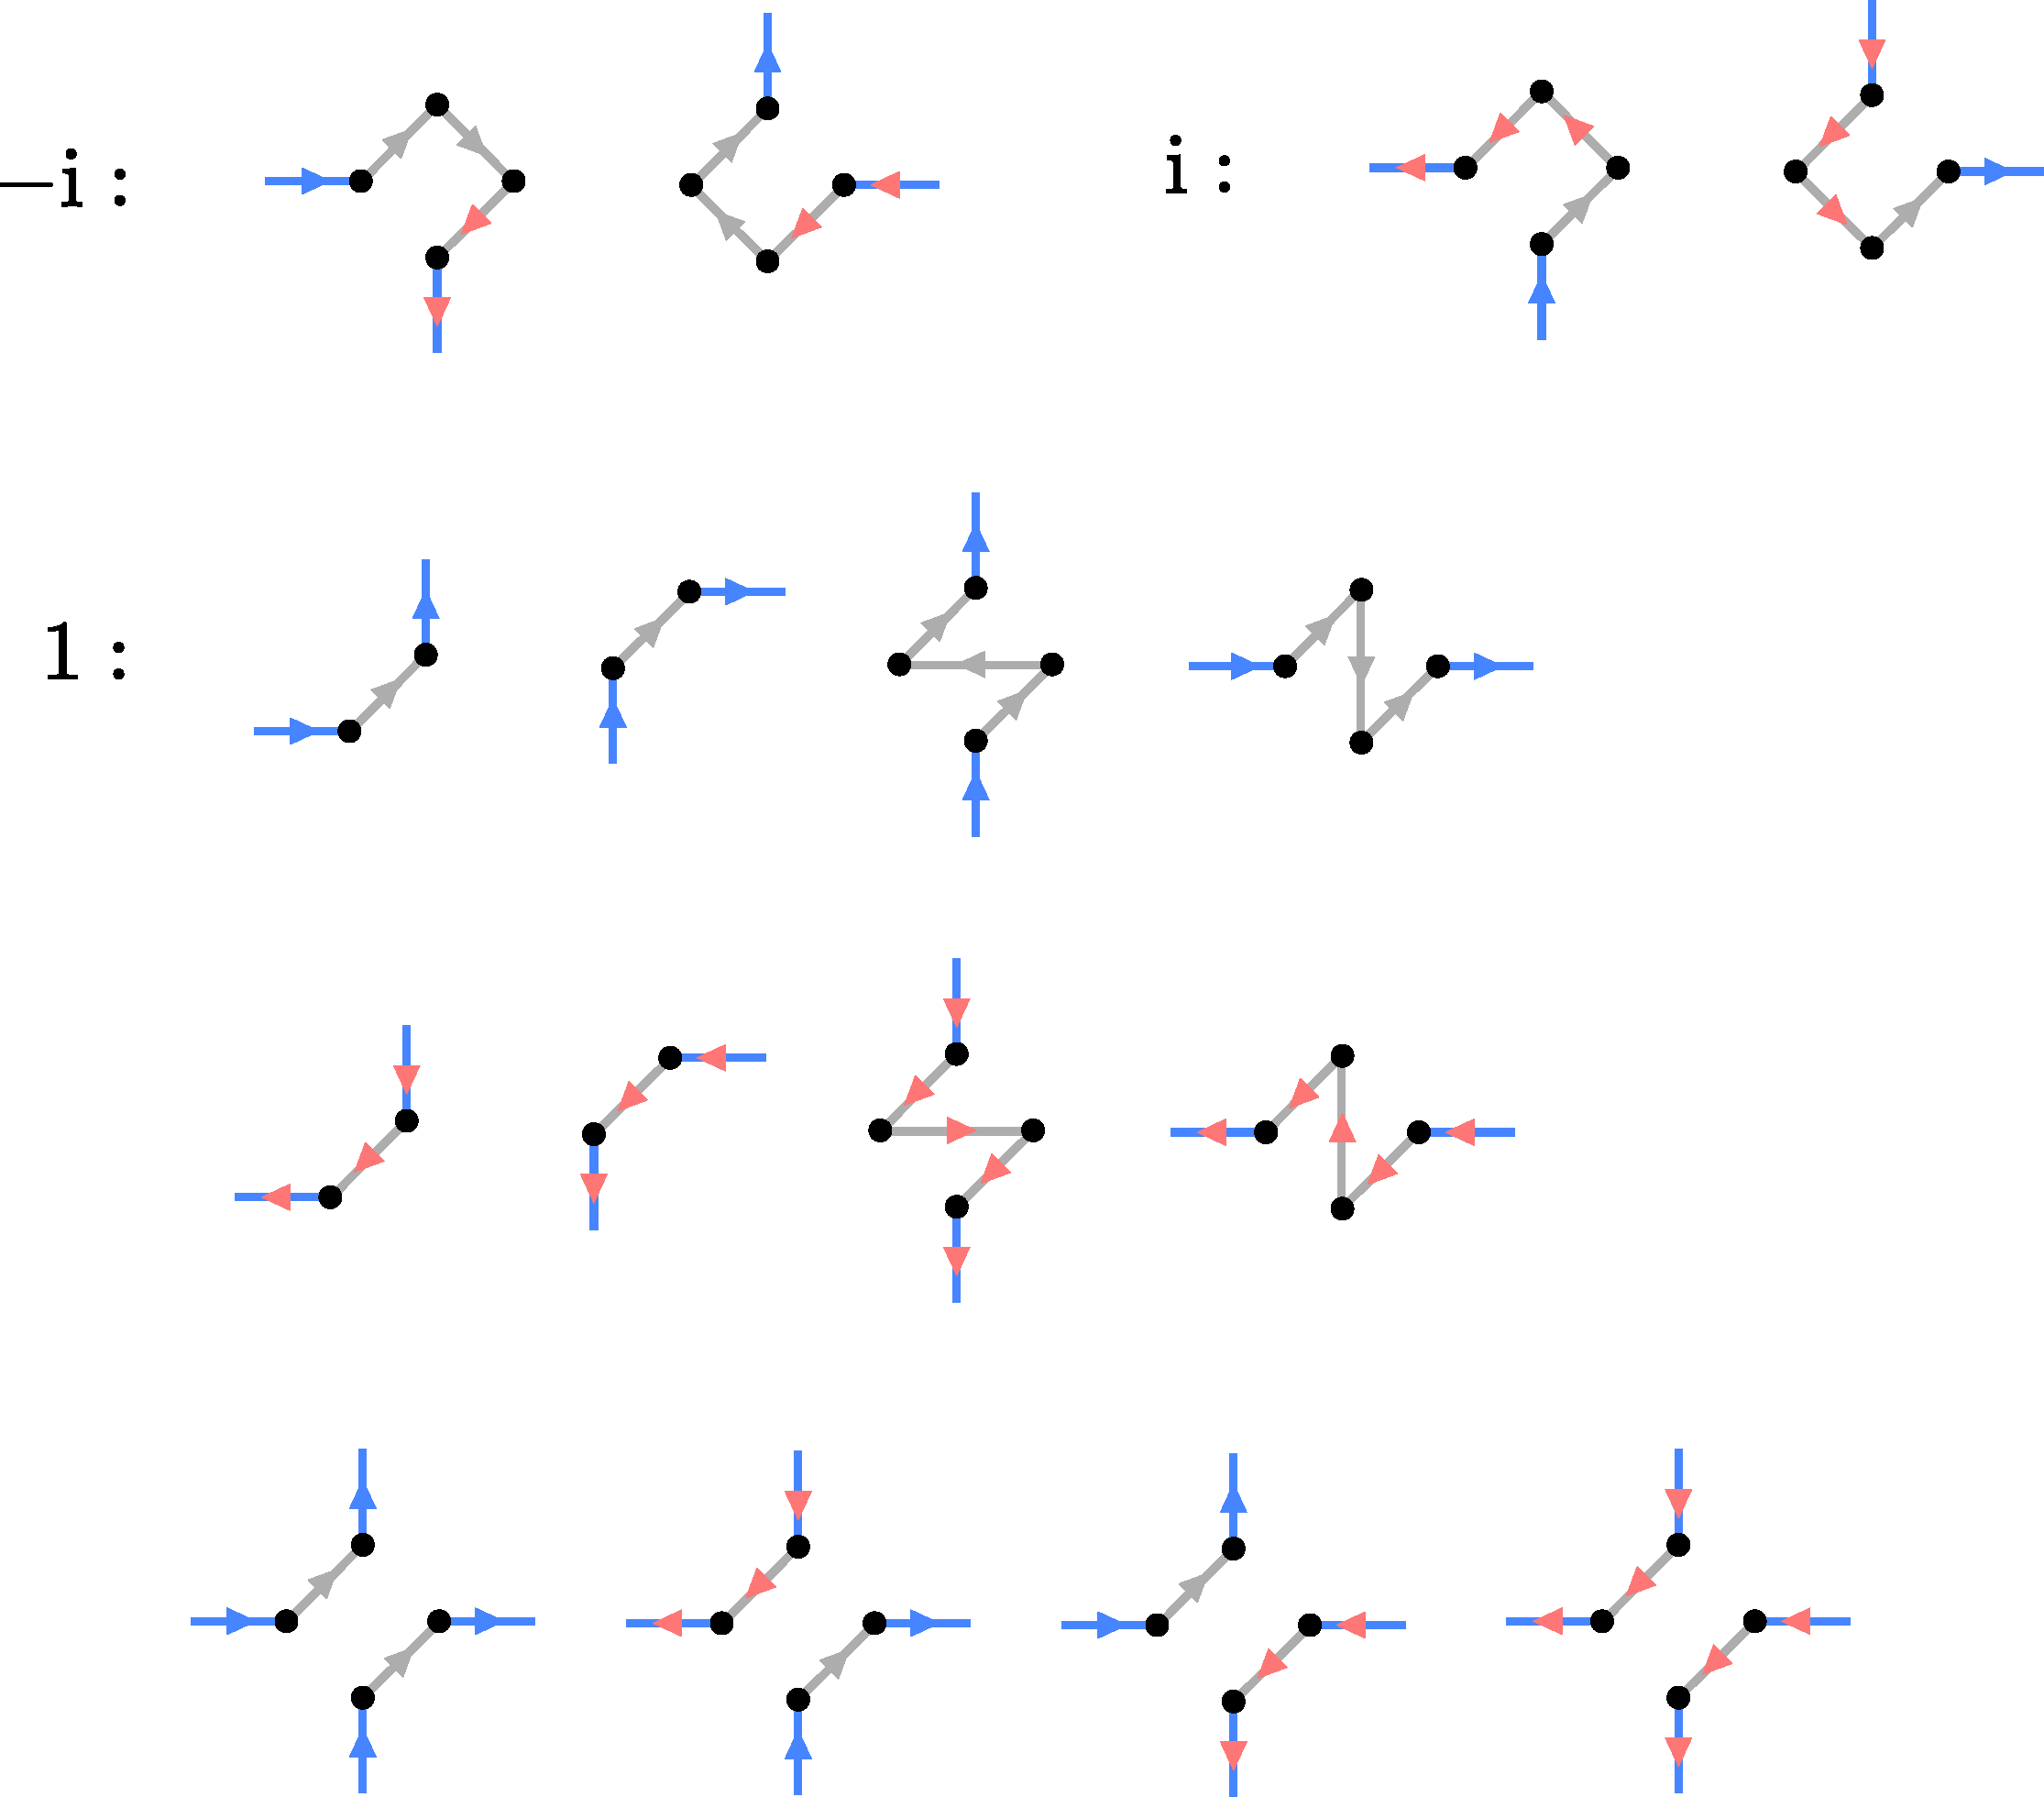
\includegraphics[width=0.7\hsize]{../images/parts.pdf}
\end{figure}
ただし、標準の向きから反転した辺を赤色で示した。
また、externalな辺は各パーツに半分ずつ含まれるので、
反転するときに$¡$を吐くとした。

非自明な符号が付くのは右上および左下を向いた角だけである。
これに注意すると、任意のダイマーの符号は$1$となることが分かる。
なぜならば、
まず長方形のサイクルに対しては$-¡$が2つでてきて、
サイクルの導入によるマイナス符号と合わせると$+1$になる。
またこの長方形を変形することで任意のサイクルが得られるが、
変形の際には必ず$±¡$がセットで出てくるため、符号は変わらない。
\begin{figure}[H]
    \centering
    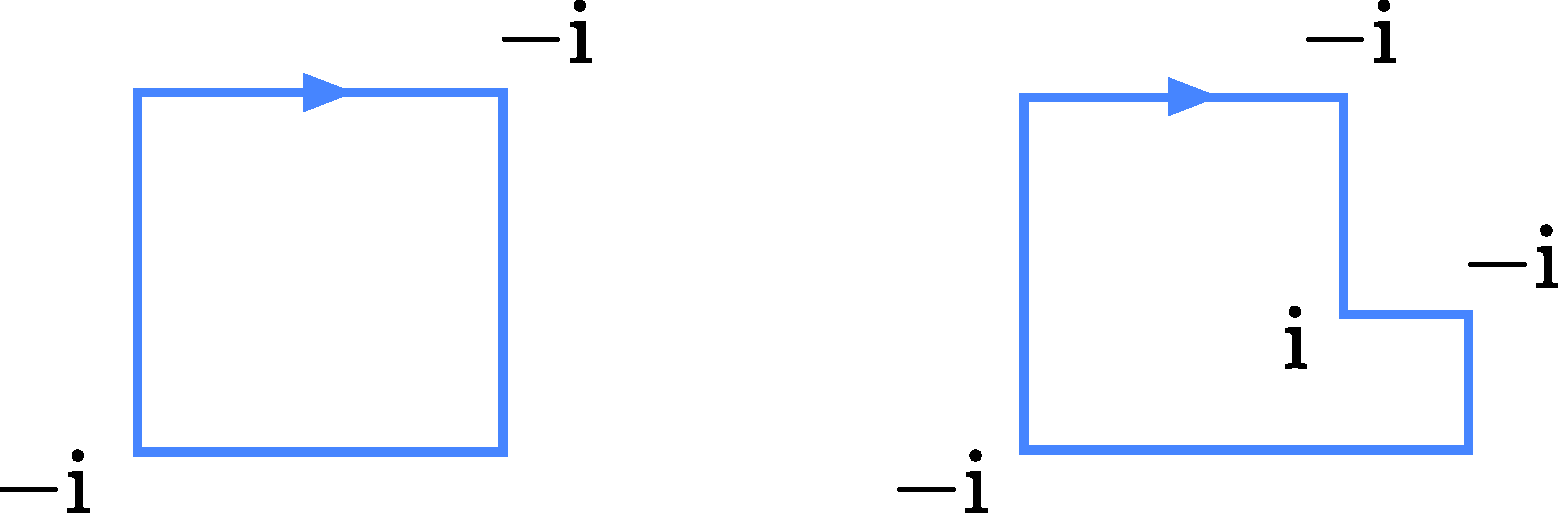
\includegraphics[width=0.4\hsize]{../images/sign.pdf}
\end{figure}
以上により、
正方格子上のサイクルの数え上げ母関数が、
ダイマーモデルの分配関数と等しいことが示された。
すなわち、
\begin{align}
    ∑_{\𝚝{closed curve}}q^{(\𝚝{length})}
    = Z_{\𝚞{Dimer}}
    = √{\det 𝒲}
\end{align}
となる。
\subsection*{
    分配関数の計算
}
ここまでで、
Isingモデルの分配関数を、
巨大な行列$𝒲 = \{w_{ij}\}$の行列式に帰着できた。
この行列式を定義どおり計算しようとすると大変だが、
$𝒲$と可換な行列に注目するとうまくいく。
今の場合明らかにサイト単位の並進対称性があるので、
並進行列の固有値によってブロック対角化ができる。
つまり、波数$(k₁,k₂)$を指定して、ベクトル
\begin{align}
    Ψ^α(x,y) = ψ^α ℯ^{¡(k₁x+k₂y)},\␣
    (x,y ∈ ℤ,~ α ∈ \{1,2,3,4\})
\end{align}
($x,y$は正方格子の添字、$α$は$K₄$の添字)
を考えると、$𝒲Ψ$も同じ波数をもつ。
したがって、
$𝒲$の波数$𝒌 = (k₁,k₂)$の部分空間に対するブロック行列を$W(𝒌)$と書くと、
\begin{align}
    ÷1{L²}\ln(∑_{\𝚝{closed curve}} q^{(\𝚝{length})})
    &
    =÷1{2L²}\ln\det 𝒲
    \∅ & 
    =÷1{2L²}∑_𝒌\ln\det W(𝒌)
    \∅ & 
    → ÷1{2}∫÷{𝑑²𝒌}{(2𝜋)²}\ln\det W(𝒌)
    \label{Z_dimer}
\end{align}
と書ける。$W(𝒌)$は具体的には以下の$4×4$行列である。
\begin{align}
    W(𝒌) = \(
              0&1+qζ₁&     -1&   -1\\
        -1-q/ζ₁&    0&      1&   -1\\
              1&   -1&      0&1+qζ₂\\
              1&    1&-1-q/ζ₂&    0
    \)
\end{align}
ただし、$ζ_j = ℯ^{¡k_j}$とした。
$ζ_j$の因子は、
externalな辺が異なるサイトの頂点をつなぐことから現れる。
この行列式を計算すると、
\begin{align}
    &
    q⁴ + (ζ₁ +÷1{ζ₁}+ ζ₂ +÷1{ζ₁})³ + 2q² 
    - (ζ₁ +÷1{ζ₁}+ ζ₂ +÷1{ζ₁})q + 1
    \∅ &
    = (q²+1)² + 2q(q²-1)(\cos k₁ +\cos k₂ )
\end{align}
となる。
したがって、
\begin{align}
    \ln\det W
    = 2\ln(q²+1) + \ln[
        1+÷{2q(q²-1)}{(q²+1)²}(\cos k₁ +\cos k₂ )
    ]
\end{align}
となる。
$q = ℯ^{-2βJ}$を代入すると、
\begin{align}
    \ln\det W = 2\ln[2q\cosh(2βJ)]
    + \ln[
        1-÷{\sinh(2βJ)}{\cosh²(2βJ)}(\cos k₁ +\cos k₂ )
    ]
\end{align}
となる。
\begin{align}
    t ≔ ÷{2\sinh(2βJ)}{\cosh²(2βJ)}
\end{align}
とおけば、(\ref{free energy with loop})、(\ref{Z_dimer})
から2次元Isingモデルの自由エネルギー
の厳密な式
\begin{align}
    -βf
    &
    = - 2\ln q + ÷1{2}∫÷{𝑑²𝒌}{(2𝜋)²}\ln\det W(𝒌)
    \∅ & 
    = 2\ln[2\cosh(2βJ)]
    + ÷1{2}∫÷{𝑑²𝒌}{(2𝜋)²}\ln[
        1 - ÷{t}2(\cos k₁ +\cos k₂)
    ]
\end{align}
を得る。
% $q=\tanh K$を代入して計算すると、
% \begin{align}
%     q²+1 = \tanh²K + 1 = ÷{\cosh 2K}{\cosh²K}
% \end{align}
% である。
% また、
% \begin{align}
%     ÷{2q(q²-1)}{(q²+1)²}
%     &
%     = 2\tanh K(\tanh²K - 1)÷{\cosh⁴K}{\cosh²2K}
%     \∅ &
%     = -÷{2\cosh K\sinh K}{\cosh²2K}
%     \∅ &
%     = -÷{\sinh 2K}{\cosh²2K}
%     ≕ -÷{t}2
% \end{align}
% である。
% したがって、(\ref{Z_dimer})から
% \begin{align}
%     ÷1{L²}\ln(∑_{\𝚝{closed curve}} q^{(\𝚝{length})})
%     = \ln(÷{\cosh 2K}{\cosh²K})
%     + ÷1{2}∫÷{𝑑²𝒌}{(2𝜋)²}\ln\𝚋[
%         1-÷t{2}(\cos k₁ +\cos k₂ )
%     ]
% \end{align}
% となる。
% この結果を(\ref{free energy with loop})に代入すると、
% \begin{align}
%     -βf = \ln(2\cosh 2K)
%     +÷1{2}∫÷{𝑑²𝒌}{(2𝜋)²}
%         \ln\𝚋[1-÷t{2}(\cos k₁ + \cos k₂)]
%     \label{free energy}
% \end{align}
% を得る。

% \section{
%     問題3
% }
% \begin{align}
%     \∂{K}(÷{2\sinh 2K}{\cosh²2K})
%     = ÷{4}{\cosh 2K} -÷{8\sinh² 2K}{\cosh³2K}
%     = 4÷{\cosh²2K-2\sinh²2K}{\cosh³2K}
% \end{align}
% \begin{align}
%     u
%     &
%     = -\∂β(-βf)
%     = -J\∂K(-βf)
%     \∅ & 
%     = -2J\tanh 2K +J∫÷{𝑑²𝒌}{(2𝜋)²}
%         ÷{}
%             {1-(t/2)(\cos k₁ + \cos k₂)}
% \end{align}

\end{document}